\documentclass{article}
\usepackage[utf8]{inputenc}
\usepackage[english]{babel}
\usepackage[T1]{fontenc}

\usepackage{graphicx}
\usepackage{amsmath}
\usepackage{amssymb}

% Title
\title{Time series exercise}
\author{Petteri Käpölä}

\begin{document}
\maketitle
\noindent
  So far we have worked with different kinds of signals assuming the sine or cosine induced seasonality in our signals. The power spectrum carries all  the information about the frequency of the phenomena we're interested in: what are the dominant frequencies in our signal and which frequencies could be categorized as 'random noise'.
  
  % Mix the answers up into a selection list
  We call a time series ordered data that is dependent on and indexed by time. For example \framebox{an audio signal}, \framebox{\texttt{sin(t)}, where \texttt{t=0:60} is a time vector} and \framebox{an EKG} are examples of time series whereas \framebox{the income distribution in 2010} and \framebox{$f(x)=x+4\sin(4x)$ where $x\in\mathbb{R}$} are not.
  
  Depending on our time series, we could be interested in the seasonality of our data: is there any and what kind of seasonality we can observe? For example, in figure \ref{fig:co2} the seasonality is very evident. In figure \ref{fig:turbulent} the seasonality is not that easily observed, if there even is any.
  
  \begin{figure}[h!]
  \centering
  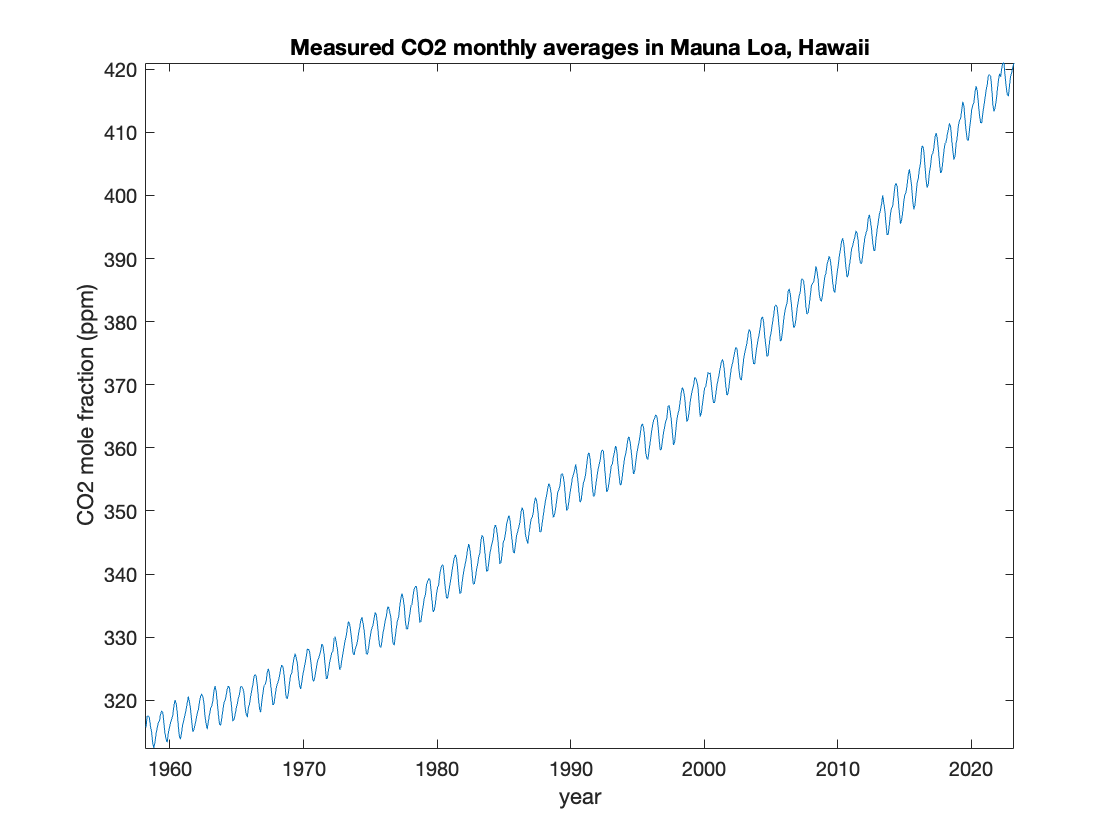
\includegraphics[width=\textwidth, height=0.75\textwidth]{co2.png}
  \caption{Very seasonal time series}
  \label{fig:co2}
  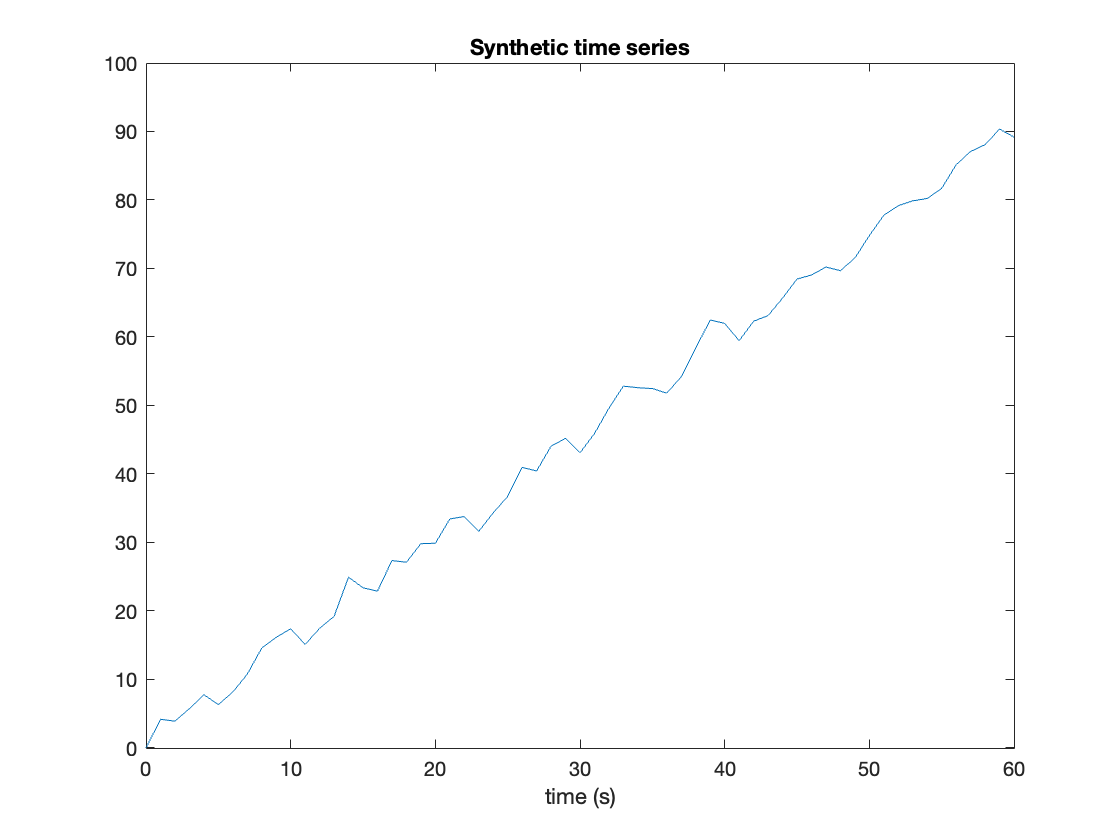
\includegraphics[width=\textwidth, height=0.75\textwidth]{turbulent.png}
  \caption{Not so seasonal time series}
  \label{fig:turbulent}
  \end{figure}
  
  Let us take a look at a time series of hourly cyclist counts in Baana, Helsinki in 2021. Read the data in with the following line of code: \\
  
  \noindent\texttt{data\_raw = readmatrix('Baana2021.xlsx');} \\
  
  We know that the counts have to be \framebox{between 0 and 1} \framebox{integers} \framebox{a continuous variable}. Also for every time index (here every hour) there \framebox{has to} \framebox{has not to} be some number of cyclists.
  
  Therefore in our data we can observe that indexes \framebox{948}, \framebox{949}, \framebox{1118}, \framebox{1140}, \framebox{1642}, \framebox{1643}, \framebox{1648}, \framebox{1649}, \framebox{1930}, \framebox{2068}, \framebox{3552}, \framebox{3762}, \framebox{4380}, \framebox{4548}, \framebox{4817} and \framebox{5578}, from smallest to largest, have unsuitable data. Before continuing, we should choose what to do with them. Fix these data points with Matlab functions \texttt{round()} and \texttt{fillmissing()} and plot the cleaned data. We can observe \framebox{a clear} \framebox{some} \framebox{no} seasonality from here.
  
  Let's then build the one-sided power spectrum of our time series using FFT as before. Set the sampling frequency to be $24$ since we have hourly data for each day of the year.
  
  The most dominant non-zero frequency value is clearly \framebox{1} and the next dominant ones are \framebox{2} and \framebox{3}. Since frequency $f$ is defined as
  
  \[f = \dfrac{1}{T},\]
  
  where $T$ is the time interval, we can express the frequency domain as time period domain by \framebox{multiplying with $T$} \framebox{taking the inverse of $f$} \framebox{taking the inverse FFT of the frequencies}. Thus we get that the most dominant oscillation happens in \framebox{$1$} $T$.
\end{document}